% Figure 1 of the paper (fig:full-system), its tikzpicture verbatim from
% main.tex in ~/src/qcaai/qce26/paper: the quantum move-selection algorithm
% as three nested levels.  The Makefile renders it to an SVG of paths, the
% way the course builds its equations.
\documentclass[dvisvgm]{standalone}
\usepackage{amsmath,amssymb}
\usepackage{tikz}
\begin{document}
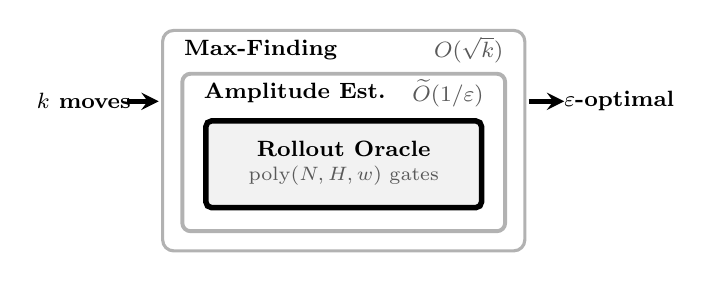
\begin{tikzpicture}[
  lbl/.style={font=\footnotesize},
  cost/.style={font=\footnotesize, text=gray!70!black},
  arr/.style={->, >=stealth, line width=0.6mm},
]
  % ── Input: k moves (text only) ──
  \node[lbl, font=\footnotesize\bfseries] at (0, -0.9) {$k$ moves};

  % arrow to Level 1
  \draw[arr] (0.55, -0.9) -- (0.95, -0.9);

  % ── Level 1: Max-Finding ──
  \draw[rounded corners=4pt, line width=0.4mm, gray!60]
    (1.0, 0.0) rectangle (5.6, -2.8);
  \node[lbl, font=\footnotesize\bfseries, anchor=west]
    at (1.15, -0.25) {Max-Finding};
  \node[cost, anchor=east] at (5.45, -0.25) {$O(\sqrt{k})$};

  % ── Level 2: Coherent Amplitude Estimation ──
  \draw[rounded corners=3pt, line width=0.5mm, gray!60]
    (1.25, -0.55) rectangle (5.35, -2.55);
  \node[lbl, font=\footnotesize\bfseries, anchor=west]
    at (1.4, -0.8) {Amplitude Est.};
  \node[cost, anchor=east] at (5.2, -0.8) {$\widetilde{O}(1/\varepsilon)$};

  % ── Level 3: Rollout Oracle (single block) ──
  \draw[fill=gray!10, rounded corners=2pt, line width=0.7mm]
    (1.55, -1.15) rectangle (5.05, -2.25);
  \node[lbl, font=\footnotesize\bfseries] at (3.3, -1.5)
    {Rollout Oracle};
  \node[cost, font=\scriptsize] at (3.3, -1.85)
    {$\mathrm{poly}(N, H, w)$ gates};

  % ── Output: ε-optimal (text only) ──
  \node[lbl, font=\footnotesize\bfseries] at (6.8, -0.9) {$\varepsilon$-optimal};

  % arrow from Level 1 to output
  \draw[arr] (5.65, -0.9) -- (6.1, -0.9);

\end{tikzpicture}
\end{document}
